% !TeX root = main.tex
\documentclass{./packages/informe}
\usepackage{./packages/caratula}
\usepackage[T1]{fontenc}
\usepackage[spanish]{babel}
\graphicspath{./files/src/.media/}

\begin{document} 

% caratula 
\titulo{TP 1: Aprendizaje supervisado}
\subtitulo{Clasificación de expresiones genómicas}
\fecha{02 de mayo, 2024}
\materia{Aprendizaje Automático}
% \grupo{Grupo 18}

\integrante{Manuel Lakowsky}{511/21}{mlakowsky@gmail.com}
\integrante{Natán Vekselman}{338/21}{natanvek11@gmail.com}
\integrante{Federico Arienti}{316/21}{fa.arienti@gmail.com}
\integrante{Kenet Chapetón}{682/19}{kenetchape@gmail.com}

\maketitle


% palabras clave y resumen
\addtocontents{toc}{\protect\setcounter{tocdepth}{0}}
\section*{resumen}
\addtocontents{toc}{\protect\setcounter{tocdepth}{3}}
Este trabajo práctico busca evaluar la aplicación de diversas técnicas y heurísticas de aprendizaje supervisado 
%---tanto en la evaluación como la construcción de distintos modelos algorítmicos--- 
para la resolución de un problema de investigación. 


En lo que sigue, evaluaremos la aplicación de los algoritmos de aprendizaje automático \textit{decision trees}, \textit{k-nearest neighbours}, \textit{linear discriminant analysis}, \textit{support vector machines}, \textit{gaussian naïve bayes} y \textit{random forests} en la construcción de un modelo predictivo; realizaremos una búsqueda de hiperparámetros prometedores para mejorar su capacidad, en términos de las métricas \textit{accuracy, auprc} y \textit{aucroc}; e investigaremos los \textit{trade-offs} entre sesgo y varianza en los modelos más prometedores. Con los resultados obtenidos, derivaremos un único clasificador y estimaremos empíricamente su poder de generalización.

% si hay tiempo: 
% Como interesa para el problema de investigación no solamente el desarrollo de técnicas de clasificación, si no también la comprensión de los resultados obtenidos, se dará especial énfasis a la \textit{interpretabilidad} de los modelos obtenidos. 

\vspace{1em}
\noindent Palabras clave: \textit{aprendizaje supervisado}, \textit{evaluación de modelos.}

% \newpage

% contenido
\vspace{1em}
\tableofcontents
\newpage

% separación de datos
\section{Separación de Datos}
Previo a realizar cualquier tipo de análisis, realizaremos un preprocesamiento de los datos. Esta tarea es crucial, ya que  permitirá estimar correctamente el poder de generalización del modelo final\footnote{Esta heurística se basa la en suposición que cualquier evaluación realizada con información accesible durante el entrenamiento puede llevar a sobreestimar la performance verdadera de un modelo, por lo que debe haber una separación entre los datos usados para la evaluación y los datos usados para el entrenamiento.}. Así también, el preprocesamiento permitirá garantizar que el entrenamiento se realice con datos lo más fieles posibles a la distribución subyacente verdadera de las clases de interés\footnote{Bajo la suposición que el dataset original es representativo de esta distribución.}. 

La idea principal es separar los datos en dos conjuntos. Por un lado, un set de entrenamiento que será utilizado para entrenar los distintos modelos a lo largo de la investigación. Por el otro, un set de evaluación, usado para medir la performance del modelo final resultante. Esta evaluación se relizará \textit{una sola vez} para garantizar que la métricas obtenidas sean lo más cercanas posible al rendimiento real, suponiendo que realizar esta evaluación de manera reiterada \textit{filtraría} información a la etapa de entrenamiento, al proveerle al investigador información de evaluación a incorporar en el modelado del pipeline de desarrollo. 

Consideramos que una buena partición, para la cantidad de datos con los que contamos, reserva entre el $10\%$ y el $20\%$ del dataset para la evaluación final, respetando la distribución de clases original en cada subconjunto. Esto se debe a que importa también maximizar la cantidad de información con la que contamos durante el entrenamiento.

Notar que, de no dividir los datos, la única opción para evaluar el rendimiento del modelo final sería utilizar los mismos datos que se utilizaron para entrenarlo. Esto es mala idea, ya que, por la misma naturaleza de los modelos, estos se acoplan en cierta medida a los datos con los que fueron entrenados. Por ejemplo, basta con que el modelo memorice las instancias de entrenamiento para obtener un rendimiento óptimo.

¿Qué instancias deberíamos incluir en cada subconjunto? Tuvimos en cuenta los siguientes factores:

\begin{itemize}
    \item La proporción de las instancias por clase debe de ser similar en cada subconjunto a la del dataset entero.
    \item La división debe ser realizada al azar para evitar cualquier estructura subyacente en los datos.
    \item Podemos asumir que los datos son independientes, en tanto sabemos que dos mediciones de RNA distintas provienen de pacientes diferentes. 
\end{itemize}

Con esto en mente, procedimos a separar los datos de la siguiente manera\footnote{Ver la función \textit{train\_test\_split} en el notebook.}:

\begin{enumerate}
    \item Dividimos el dataset $D$ entre instancias positivas ---\textit{buen pronóstico} $=1$--- y negativas ---\textit{mal pronóstico} $=0$---. Las desordenamos al azar con un algoritmo de shuffle\footnote{Usamos el generador \textit{default\_rng} de \textit{numpy.random}, con un valor de semilla para permitir la reproducción de los resultados.}: $$D \rightarrow (P, N)$$
    \item Separamos el último $10\%$ de cada grupo, obteniendo los datos de entrenamiento y evaluación: $$P \rightarrow (P_{train}, P_{test})\ \ \ \text{y}\ \ \ N \rightarrow (N_{train}, N_{test})$$.
    \item Obtuvimos los conjuntos finales concatenando las listas del mismo tipo y, nuevamente, los desordenamos al azar: $$(D_{train}, D_{test}) = (P_{train} \cup N_{train},\ P_{test} \cup N_{test})$$
\end{enumerate}

\vspace{0.5em}
La división se puede observar en la Figura \ref{distribucion}. Las probabilidades fueron truncadas, en vez de redondeadas, para capturar las pequeñas variaciones existentes. El valor de semilla utilizado fue $s = \text{0x2031}$, el mismo se utilizará para controlar todos los procesos aleatorios a lo largo de este trabajo.

\vspace{0.5em}
\begin{figure}[!htbp]
    \begin{center}
        \begin{tabular}{ |c|c|c|c| } 
         \hline
                    & $D$      & $D_{train}$ & $D_{test}$ \\
        \hline
        $P(y=1)$   & $0.3140$ & $0.3140$    & $0.3137$   \\ 
        $P(y=0)$   & $0.6860$ & $0.6859$    & $0.6862$   \\ 
        $n$        & $500$    & $449$       & $51$       \\ 
        \hline
        \end{tabular}
    \end{center}
    \caption{Distribución de clases y tamaños del split del dataset $D$ en entrenamiento ---$D_{train}$--- y evaluación ---$D_{test}$---.} \label{distribucion}
\end{figure}


% construcción de un modelo simple
\section{Construcción de modelos}
\subsection{Un árbol de decisión simple}\label{simple}

Como punto de partida para nuestro análisis, vamos a entrenar un \textit{árbol de decisión} simple sobre los datos de entrenamiento. De esta manera, tendremos un piso respecto a la performance que podemos esperar de cualquier modelo a entrenar. Con \textit{simple} nos referimos a un modelo de poca complejidad, que sea fácilmente interpretable y propenso a subestimar por contar con un sesgo inductivo alto\footnote{En otras palabras, cuyo espacio de hipótesis sea sencillo.}. De manera concreta, el árbol a entrenar tendrá una profundidad máxima de $3$ niveles y usará los hiperparámetros por defecto de la biblioteca \textit{scikit-learn}\footnote{Luego, las hipótesis representables tendrán la forma de conjunciones de a lo sumo tres comparaciones, donde cada comparación evalúa algún umbral para algún atributo particular de las instancias.} para el \textit{DecisionTreeClassifier}.

Para estimar la performance del modelo utilizaremos $5$-fold cross validation estratificado\footnote{Ver la función \textit{cross\_val} en el notebook adjunto. Usamos el splitter \textit{StratifiedKFold} de \textit{scikit-learn}, con \textit{random\_state} $= s$. Para procurar que la comparación entre métricas sea justa, se reseteó el \textit{random\_state} entre corridas.} sobre $D_{train}$, para las métricas de \textit{accuracy}, \textit{aucroc} y \textit{auprc}. Mediremos la performance en entrenamiento y validación por split. También, tomaremos el promedio $\bar\phi$ en ambos casos y, para validación, realizaremos el cálculo del score global\footnote{Notar que todo $D_{train}$ fue parte del set de validación para alguna iteración de cross validation. Luego, podemos calcular $$\Phi = metrica(\bigcup_{i=1}^5\text{Predict}(M^{(i)}, X_{cv_{validation}}^{(i)}), y_{train})$$ para estimar la performance del modelo sin recurrir a promedios.} $\Phi$.

% \vspace{0.5em}
% \begin{enumerate}
%     \item Dividimos el set de entrenamiento en $5$ grupos al azar, procurando que cada grupo mantenga la distribución de clases del set original\footnote{Usamos el splitter \textit{StratifiedKFold} de \textit{scikit-learn} con $k=5$ y \textit{random\_state} $= s$. Para procurar que la comparación entre métricas sea justa, se reseteó el \textit{random\_state} entre corridas.}: $$D_{train} \rightarrow (D_{train}^{(1)}, D_{train}^{(2)}, D_{train}^{(3)}, D_{train}^{(4)}, D_{train}^{(5)})$$
% 
%     \item Por turnos, consideramos un subconjunto como un set de \textit{validación} y al resto como un set de \textit{entrenamiento}.$$
%     cv^{(i)} = (D_{cv_{train}}^{(i)},\ D_{cv_{validation}}^{(i)}) = (D_{train}^{(i)},\ \bigcup_{j \neq i} D_{train}^{(j)})\ \ \forall i: 1 \dots 5$$
% 
%     \item Por cada par $cv^{(i)} $, entrenamos un \textit{árbol de decisión} simple, con los hiperparámetros descriptos: $$M^{(i)} = \text{Train}(Arbol,\ D_{cv_{train}}^{(i)})$$
%     
%     \item Evaluamos la performance de cada modelo $M^{(i)}$ sobre $cv^{(i)}$, utilizando la métrica seleccionada: 
%     \begin{align*}
%         \phi_{train}^{(i)} &= \text{metric}(\text{Predict}(M^{(i)}, X_{cv_{train}}^{(i)}), y_{cv_{train}}^{(i)})\\
%         \phi_{validation}^{(i)} &= \text{metric}(\text{Predict}(M^{(i)}, X_{cv_{validation}}^{(i)}), y_{cv_{validation}}^{(i)})
%     \end{align*}
%     \item Tomamos el promedio de las evaluaciones, para tener un primer estimado del desempeño del modelo, independiente de $D_{train}$. Es decir, un estimación \textit{realista} de la performance:
%     \begin{align*}
%         \bar{\phi}_{train} &= \frac{1}{5}\sum_{i=1}^{5} \phi_{train}^{(i)}\\
%         \bar{\phi}_{validation} &= \frac{1}{5}\sum_{i=1}^{5} \phi_{validation}^{(i)}
%     \end{align*}
%          
%     \item Evaluamos la métrica sobre el conjunto total de datos\footnote{Notar que todo el conjunto fue parte del set de validación para alguna iteración.}, para tener otro estimado del desempeño del modelo, independiente de $D_{train}$:
%     \begin{align*}
%         \Phi_{validation} &= metric(\bigcup_{i=1}^5\text{Predict}(M^{(i)}, X_{cv_{validation}}^{(i)}), y_{train})
%     \end{align*}
% \end{enumerate}
%\vspace{0.5em}

Los resultados se pueden observar en las Figuras \ref{metricas_simple} y \ref{curvas_simple}. Como es esperable, la performance sobre entrenamiento es más alta que la performance sobre validación, para todas las métricas. El hecho que no se logren valores muy altos en entrenamiento da cuenta de un problema de sesgo, como ya habíamos previsto.

\vspace{0.5em}
\begin{figure}[!htbp]
\begin{center}
\begin{tabular}{ |c|c|c|c|c|c|c| } 
\hline
            & accuracy  & accuracy      & auprc     & auprc         & aucroc   & aucroc      \\
            & (train)   & (validación)  & (train)   & (validación)  & (train)   & (validación) \\      
\hline
i=1         & $0.8329$  & $0.7333$      & $0.7676$  & $0.5019$      & $0.7869$  & $0.6270$ \\
i=2         & $0.8189$  & $0.6556$      & $0.7618$  & $0.3545$      & $0.8103$  & $0.6342$ \\
i=3         & $0.8245$  & $0.6333$      & $0.7689$  & $0.5603$      & $0.8460$  & $0.6699$ \\
i=4         & $0.8189$  & $0.7000$      & $0.7551$  & $0.4572$      & $0.7890$  & $0.6221$ \\
i=5         & $0.8083$  & $0.7303$      & $0.7820$  & $0.5590$      & $0.8662$  & $0.6537$ \\
$\bar\phi$  & $0.8207$  & $0.6905$      & $0.7671$  & $0.4869$      & $0.8197$  & $0.6414$ \\
$\Phi$      & -         & $0.6904$      & -         & $0.4810$      & -         & $0.6590$ \\
\hline
\end{tabular}
\end{center}
\caption{Resultados de $5$-fold cross validation estratificado sobre los datos de entrenamiento para las métricas de \textit{accuracy}, \textit{aucroc} y \textit{auprc}, redondeados a cuatro dígitos significativos.}\label{metricas_simple}
\end{figure}

\begin{figure}[!htbp]
    \centering 
    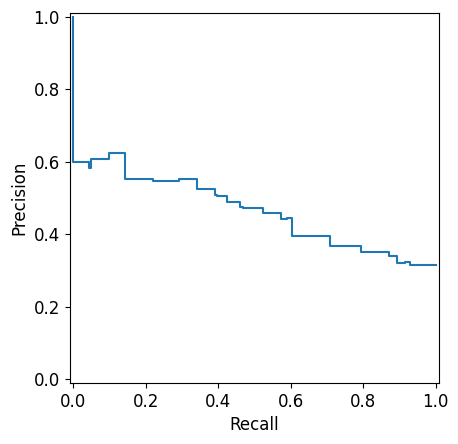
\includegraphics[width=0.45\textwidth]{/files/src/.media/simpleTreeAuprc.png}
    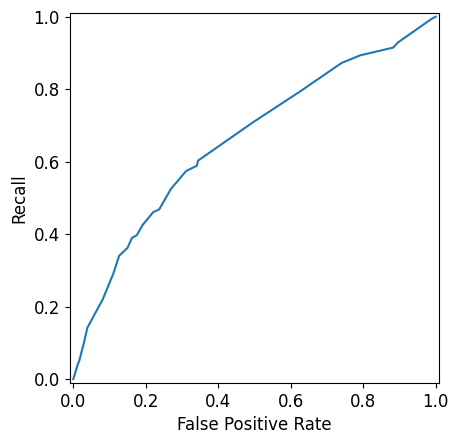
\includegraphics[width=0.45\textwidth]{/files/src/.media/simpleTreeAucroc.png}
    \caption{Curvas \textit{precision-recall}, izquierda, y \textit{receiving operator characteristic}, derecha, para el árbol de decisión \textit{simple}.}
    \label{curvas_simple}
\end{figure}

Tal vez no sorprendentemente, desde el punto de vista de \textit{aucroc}, el modelo funciona apenas un poco mejor que tomar una decisión aleatoria.

Es interesante notar que \textit{accuracy} obtuvo un valor más alto que \textit{auprc} y \textit{aucroc} en validación. Esto puede dar cuenta de la incapacidad de \textit{accuracy} para capturar el efecto de los distintos tipos de errores en un problema con clases desbalanceadas. También, parece interesante que tanto \textit{accuracy} como \textit{auprc} obtuvieron en validación resultados más variados que \textit{aucroc}: \textit{auprc} varió hasta un $\approx 20\%$ entre splits.

Un detalle importante en la interpretación de estos resultados, creemos, es la importancia sobre la decisión de \textit{cuál es la clase positiva}. En particular, \textit{auprc} está sesgado hacia el comportamiento de esta clase, mientras que \textit{aucroc} es más imparcial \cite{Saito}. 


\subsection{Búsqueda en cuadrícula}

Dados los resultados, parece interesante explorar otros hiperparámetros para estimar qué tan capaces pueden llegar a ser los \textit{árboles de decisión} para el problema bajo estudio. Para ello, realizaremos una primer búsqueda en cuadrícula con algunos hiperparámetros provistos por la cátedra. En la próxima sección lo complementaremos con una búsqueda aleatoria más extensiva.

En este caso, evaluaremos las combinaciones de hiperparámetros que titulan la Figura \ref{grid_search}, aplicando $5$-fold cross validation estratificado con métrica \textit{accuracy} promedio\footnote{Por decisión de la cátedra para este ejercicio.}.

\vspace{0.5em}
\begin{figure}[!htbp]
    \begin{center}
        \begin{tabular}{ |c|c|c|c| } 
         \hline
        Altura Máxima   & Criterio de corte & Accuracy (train)  & Accuracy (validación) \\
        \hline
        $3$             & Gini              &  $0.8207$         & $0.6905$  \\ 
        $5$             & Gini              &  $0.9126$         & $0.7127$  \\
        $\infty$        & Gini              &  $1.0000$         & $0.6637$  \\ 
        $3$             & Entropía          &  $0.7890$         & $0.6815$  \\
        $5$             & Entropía          &  $0.8937$         & $0.6503$  \\ 
        $\infty$        & Entropía          &  $1.0000$         & $0.6459$  \\ 
        \hline
        \end{tabular}
    \end{center}
    \caption{\textit{Accuracy} promedio resultante de realizar $5$-fold cross validation estratificado, para \textit{árboles de decisión} con distintos hiperparámetros.} \label{grid_search}
\end{figure}

La figura \ref{grid_search} muestra los resultados obtenidos. Podemos ver una clara tendencia a sobreajustar a medida que aumenta la altura máxima permitida. Por su parte, el criterio Gini obtuvo mejores resultados que Entropía en todas las instancias de evaluación. Algo que llama la atención es que un aumento modesto en la altura máxima permitida (de $3$ a $5$ niveles) causó una mejora en evaluación al usar el criterio Gini, pero una pérdida en el caso de Entropía.


\vspace{1em}
\section{Comparación de algoritmos}
A partir de los resultados del árbol \textit{simple}, interesa explorar el uso de distintos algoritmos de aprendizaje que puedan arrojar mejores resultados. En particular, evaluaremos la performance de los \textit{árboles de decisión}, \textit{k-nearest neighbours}, \textit{linear discriminant analysis}, \textit{support vector machines} y \textit{gaussian naïve bayes} en términos de \textit{aucroc} promedio. Para cada uno, realizaremos una búsqueda aleatoria con el objetivo de encontrar buenos hiperparámetros, guiados por nuestras propias suposiciones respecto a cuáles pueden llegar a importar y en qué rangos de valores.

La búsqueda se realizará con \textit{RandomizedSearchCV} de \textit{scikit-learn}, utilizando como mecanismo de evaluación $5$-fold cross-validation estratificado. Se harán $100$ iteraciones por algoritmo.

\subsection{Árboles de decisión}
Para este clasificador, se considerarán los siguientes hiperparámetros y rangos. 

\begin{itemize}
    \item El criterio de corte: permitimos todos los criterios implementados por el algoritmo. Estos son \textit{Gini}, \textit{Entropy} y \textit{Log loss}. 
    \item La profundidad máxima: permitimos que varie en el rango $[3,\ \lfloor\sqrt{n} \rfloor]$ de manera uniforme, con $n=451$, bajo la suposición que un árbol \textit{corto} es preferible tanto a un \textit{stump} como a un árbol profundo.
    \item La cantidad de atributos máxima a considerar por corte: permitimos que varíe de manera uniforme sobre $[1, p]$, con $p = 200$.
\end{itemize}

Si bien se exploraron de manera tentativa otros hiperparámetros, se decidió no agregarlos a la búsqueda general, ya que  parecían no influir positivamente en los resultados. Basamos esta idea, también, en que consideramos que la cantidad de restricciones agregadas es inversamente proporcional a la probabilidad de encontrar una buena combinación de hiperparámetros, en especial cuando la influencia de los hiperparámetros no pareceria ser igual. 

La Figura \ref{random_tree} muestra los $5$ mejores candidatos obtenidos. Los resultados respaldan la supocisión de que un árbol corto es mejor a uno profundo (notar que $\lfloor\sqrt{n} \rfloor = 21$).

\vspace{0.5em}
\begin{figure}[!htbp]
    \begin{center}
        \begin{tabular}{ |c|c|c|c| } 
         \hline
        Altura Máxima   & Criterio de corte & Atributos Máximos  & aucroc (validación) \\
        \hline
        $3$             & Entropía          &  $135$            & $0.6843$  \\ 
        $3$             & Entropía          &  $14$             & $0.6598$  \\
        $4$             & Log loss          &  $148$            & $0.6517$  \\ 
        $3$             & Log loss          &  $77$             & $0.6513$  \\
        $9$             & Entropía          &  $91$             & $0.6468$  \\ 
        \hline
        \end{tabular}
    \end{center}
    \caption{mejores resultados para la búsqueda aleatoria de hiperparámetros en el caso de \textit{árboles de decisión}.} \label{random_tree}
\end{figure}

Si bien el criterio de corte influye, la similitud entre Gini y Entropía llevan a intuir que fue la limitación en la cantidad máxima de atributos a considerar la que llevó a una mejora sustancial con respecto al modelo de la Sección \ref{simple}. Esto puede deberse a que limita la influencia de los atributos más importantes durante la construcción del árbol.

\subsection{K-Nearest neighbours}
En este caso, se utilizará el clasificador \textit{KNeighborsClassifier} de \textit{scikit-learn} con las siguientes opciones de hiperparámetros.

\begin{itemize}
    \item Cantidad de vecinos más cercanos: permitimos que sigan una distribución \textit{LogUniform(10, n/2)}. La cota inferior de $10$ porque para valores más bajos no encontramos evidencia empírica que mejore la performance. 
    \item Eleccion de pesos por vecino: Permitimos \textit{Uniform} donde cada instancia se pondera por igual, o \textit{Distance} donde los vecinos más cercanos tendrán un peso más determinante que los demás.
    \item Eleccion de metrica: Optamos que se usen las métricas usuales \textit{l1}, \textit{l2}, \textit{l3} y \textit{l4}. 
\end{itemize}

Se seleccionó una distribución \textit{LogUniforme} para determinar el valor de kk, dado que resulta conveniente evitar valores excesivamente grandes, los cuales podrían inducir overfitting. Al generar 100 muestras de esta distribución y establecer una cota inferior adecuada, se busca controlar el riesgo de underfitting.

Observando la Figura \ref{knn}, se identificó que la elección de pesos ponderados basados en la distancia, combinados con la métrica 1 (l1), pareciera ser óptima para el problema en cuestión.
Además, la búsqueda aleatoria permitió determinar un rango apropiado de vecinos, comprendido entre 10 y 30.
\vspace{0.5em}
\begin{figure}[!htbp]
    \begin{center}
        \begin{tabular}{ |c|c|c|c| } 
         \hline
        N   & Eleccion de pesos & P  & aucroc (validación) \\
        \hline
        $15$             & Distance          &  $1$             & $0.8391$  \\ 
        $11$             & Distance          &  $1$             & $0.8386$  \\
        $14$             & Distance          &  $1$             & $0.8375$  \\ 
        $13$             & Distance          &  $1$             & $0.8360$  \\
        $26$             & Distance          &  $1$             & $0.8287$  \\ 
        \hline
        \end{tabular}
    \end{center}
    \caption{mejores resultados para la búsqueda aleatoria de hiperparámetros para \textit{k-nearest neighbours}.} \label{knn}
\end{figure}

\subsection{Linear discriminant analysis}
La busqueda, para el clasificador \textit{LinearDiscriminantAnalysis} de \textit{scikit-learn} fue llevada a cabo con los siguientes hiperparámetros: 

\begin{itemize}
    \item Solver: Permitimos los algoritmos basados en \textit{LSQR}, \textit{SVD} y \textit{EIGEN}.
    \item El metodo de contraccion: Cuando no se este usando SVD, permitimos que siga una distribucion $Uniforme(0,1)$.
\end{itemize}

Se exploraron otros hiperparámetros, pero optamos por no agregarlos debido a que no parecian influir de forma significativa en los resultados finales. 

Al observar la Figura \ref{lda}, notamos que la elección del Solver (Eigen o Lsqr) parece no influir significativamente. Más bien, resulta más determinante el uso de un parámetro de contracción adecuado, que parece rondar los $0.26$. Finalmente, se observa que el uso de SVD no conduce a una buena performance.

\vspace{0.5em}
\begin{figure}[!htbp]
    \begin{center}
        \begin{tabular}{ |c|c|c|c| } 
         \hline
        Solver   & Shrinkage & auc-roc (validación) \\
        \hline
        eigen                   &  0.270007          & $0.8648$  \\ 
        lsqr                    &  0.272309          & $0.8648$  \\
        lsqr                    &  0.266565          & $0.8648$  \\ 
        lsqr                    &  0.274341          & $0.8647$  \\
        eigen                   &  0.288274          & $0.8645$  \\ 
        \hline
        \end{tabular}
    \end{center}
    \caption{Mejores resultados para la búsqueda aleatoria de hiperparámetros para \textit{linear discriminant analysis}.} \label{lda}
\end{figure}

\subsection{Support vector machines}
Realizamos la busqueda, para el modelo \textit{Support Vector Machines}. Llevada a cabo con el clasificador \textit{SVC} de \textit{scikit-learn}, usamos los siguientes hiperparámetros y rangos: 

\begin{itemize}
    \item Parámetro de regularización: Optamos porque siga una distribucion \textit{LogUniform(1e-5,1e2)}, como el valor es inversamente proporcional a `C` es relevante que tome mas valores chicos que grandes pues hara que la suma poderada de errores de las instancias que estan en el lado equivocado de la frontera de decision, tenga un grado mas de tolerancia.
    \item Kernel: Permitimos \textit{linear}, \textit{poly}, \textit{rbf} (función de base radial) y \textit{sigmoid} (función tanh).
    \item Coeficiente de Kernel: Decidimos elegir entre \textit{scale}, que toma $ \gamma = \frac{1}{p*X.var()}$, u \textit{auto} con $\gamma = \frac{1}{p} $, donde $p=200$ (cantidad de genes).
\end{itemize}

En la Figura \ref{support vector machines}, se observa que la configuración más relevante, a priori, es que $\gamma$ este escalado, que busca normalizar la influencia de las características en el cálculo de la función de kernel. Esta normalización es especialmente útil para conjuntos de datos que contienen características de diferentes escalas. Además, se destaca que el kernel de función de base radial resultó ser el más exitoso. Aunque no parece que el parámetro C tenga una influencia significativa, los valores seleccionados no fueron muy grandes. Es importante señalar que los grados solo se consideran en los kernels \textit{poly}; por lo tanto, no tienen relevancia para los demás tipos de kernel.
\vspace{0.5em}
\begin{figure}[!htbp]
    \begin{center}
        \begin{tabular}{ |c|c|c|c|c| } 
         \hline
        $C$ & Kernel & $\gamma$ & grado & aucroc (validación) \\
        \hline
        $2.5408$ & rbf     & scale & $7$ & $0.8960$ \\ 
        $2.6202$ & rbf    & scale & $6$ & $0.8960$ \\
        $13.4965$ & rbf   & scale & $3$ & $0.8956$ \\ 
        $20.2985$ & rbf   & scale & $8$ & $0.8956$ \\
        $3.4142$ & rbf    & scale & $6$ & $0.8955$ \\ 
        \hline
        \end{tabular}
    \end{center}
    \caption{mejores resultados para la búsqueda aleatoria de hiperparámetros para \textit{support vector machines}.} \label{support vector machines}
\end{figure}

\subsection{Gaussian naïve bayes}
Se examinó por último el rendimiento del clasificador \textit{GaussianNB} de \textit{scikit-learn}. Los hiperparámetros de este algoritmo a optimizar y sus rangos fueron:

\begin{itemize}
    \item Las probabilidades a priori de las clases: permitimos que varíen de manera normal con \textit{media} igual a las probabilidades a priori empíricas (ver Figura \ref{distribucion}) y una \textit{desviación estándar} de $\sigma = 0.1$.
    \item El suavizado de varianza: permitimos que varíe uniformemente en el rango $[0, 1 \times 10^{-2}]$.
\end{itemize}

Como valor predeterminado, \textit{GaussianNB} considera las \textit{probabilidades a priori} de cada clase como sus respectivas proporciones en el dataset. Para ampliar el rango de búsqueda, en lugar de usar las probabilidades originales se utilizaron valores aleatorios cercanos a estas.

Por otro lado, el \textit{suavizado de varianza} indica la cantidad que se suma a todas las varianzas de los atributos para evitar que sean cero\footnote{Su valor representa el porcentaje de la varianza más alta a sumarle a todas las demás.}, lo cual podría producir errores numéricos durante el cálculo de las distribuciones normales. Aunque tiene un valor predeterminado de $1 \times 10^{-9}$, probamos con números al azar hasta $1 \times 10^{-2}$.

Al observar la Figura \ref{naive_bayes}, podemos destacar dos hallazgos interesantes. En primer lugar, parece que el algoritmo tiene baja varianza, ya que al cambiar significativamente las proporciones de las etiquetas su capacidad predictiva se mantiene estable. Por otro lado, da la impresión de que el mejor valor para el suavizado de la varianza de los atributos se encuentra cerca de la cota superior de la búsqueda, es decir, $1 \times 10^{-2}$. Al dejar su valor predeterminado de $1 \times 10^{-9}$, el mejor puntaje obtenido fue de $0.785$, aproximadamente un $7\%$ de reducción respecto a los de la tabla.

\vspace{0.5em}
\begin{figure}[!htbp]
    \begin{center}
        \begin{tabular}{ |c|c|c|c| } 
         \hline
        $P(Y=0)$ & $P(Y=1)$ & Suavizado & aucroc (validación) \\
        \hline
        $0.6320$ & $0.3680$ & $0.975 \times 10^{-2}$ & $0.8408$ \\ 
        $0.6119$ & $0.3881$ & $0.973 \times 10^{-2}$ & $0.8408$  \\
        $0.6579$ & $0.3421$ & $0.982 \times 10^{-2}$ & $0.8406$  \\ 
        $0.8183$ & $0.1817$ & $0.980 \times 10^{-2}$ & $0.8406$  \\
        $0.5157$ & $0.4843$ & $0.960 \times 10^{-2}$ & $0.8406$  \\ 
        \hline
        \end{tabular}
    \end{center}
    \caption{mejores resultados para la búsqueda aleatoria de hiperparámetros para \textit{naïve bayes}.} \label{naive_bayes}
\end{figure}



\vspace{1em}
\section{Diagnóstico Sesgo-Varianza}
% En este punto, se pide inspeccionar **tres** de sus mejores modelos encontrados hasta ahora de cada familia de modelos: la mejor configuración para el árbol de decisión, la mejor configuración para LDA y la mejor configuración para SVM. Para ello:

% 1. Graficar curvas de complejidad para cada modelo (excepto para LDA), variando la profundidad en el caso de árboles, y el hiperparámetro C en el caso de SVM. Diagnosticar cómo afectan al sesgo y a la varianza esos dos hiperparámetros.
% 2. Graficar curvas de aprendizaje para cada modelo. En base a estas curvas, sacar conclusiones sobre si los algoritmos parecen haber alcanzado su límite, o bien si aumentar la cantidad de datos debería ayudar.
% 3. Construir un modelo **RandomForest** con 200 árboles. Explorar para qué sirve el hiperparámetro max_features y cómo afecta a la performance del algoritmo mediante una curva de complejidad. Explicar por qué creen que se dieron los resultados obtenidos. Por último, graficar una curva de aprendizaje sobre los parámetros elegidos para determinar si sería útil o no conseguir más datos.

% **Atención**: Tener en cuenta que debemos seguir utilizando AUC ROC como métrica para estas curvas.

% Para cada método pueden incluir hasta una carilla de texto y los gráficos que considere relevantes.

Procedemos en esta sección a inspeccionar los mejores modelos encontrados para los clasificadores \textit{árboles de decisión}, \textit{LDA} y \textit{SVM}. En particular, buscamos entender su comportamiento al aumentar su complejidad (variando alguno de sus hiperparámentros), trazar sus curvas de aprendizaje, y sacar conclusiones sobre sus varianzas y sesgo. Por último, los compararemos con un clasificador de tipo \textit{random forest}.

\subsection{Árboles de decisión}
Para el mejor modelo obtenido en la Figura \ref{random_tree}, variamos la \textit{profundidad máxima} para graficar las curvas de complejidad observadas en la Figura \ref{decisionTreeComplexity}. En ella podemos apreciar que, a partir de los clasificadores de \textit{altura máxima} $> 7$, el modelo se acopla completamente a los datos de entrenamiento, generando un \textit{overfitting}. A su vez, sus respectivas performances en los datos de validación decrementan desde el mejor valor de $\textit{altura máxima} = 4$ hasta estabilizarse en las alturas mayores a 8. Esto podría indicar que el modelo ya separó todas las instancias en sus respectivas hojas, y dejó de cambiar sus reglas de corte. Podemos también apreciar que durante la búsqueda aleatoria de hiperparámentros la combinación con \textit{altura máxima} 4 no se habría probado, de otro modo hubiese aparecido como la mejor.  
\begin{figure}[!htbp]
    \centering
    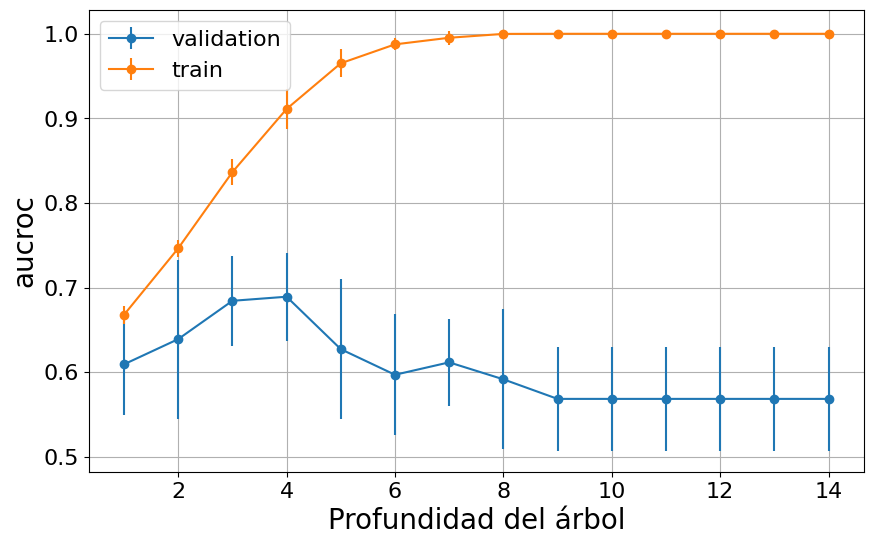
\includegraphics[width=0.75\textwidth]{/files/src/.media/decisionTreeComplexity.png}
    \caption{Curvas de complejidada para el clasificador \textit{decision tree}, mostrando la variación del AUC ROC en datos de entrenamiento y validación a medida que se aumenta su profundida máxima. Las lineas verticales denotan la varianza para cada valor del atributo.}
    \label{decisionTreeComplexity}
\end{figure}

Con respecto a la varianza, podemos observar que el rendimiento de los modelos varía considerablemente según el dataset utilizado en entrenamiento. Esto puede apreciarse en las barras de error\footnote{Estas provienen de las mediciones de AUC ROC para cada fold de validación.}, donde en algunos casos como para \textit{altura máxima} = 2 y 5, hubo una diferencia de performance en más de un $10\%$. A su vez, puede verse cómo se van separando ambas curvas a medida que aumenta la profundidad máxima. Es decir, la performance del modelo en entrenamiento aumenta al hacer \textit{overfitting} mientras que en validación decrece. Esto muestra que la varianza del clasificador crece junto con la profundidad máxima, ya que el modelo se acopla cada vez más al dataset.

Por otro lado, todos los resultados del algoritmo en validación se encuentran con un AUC ROC por debajo de $0.75$, y con media aproximadamente en $0.6$, con lo cual parecería tener poca capacidad predictiva. En ese sentido, sin importar el valor del hiperparámentro parecería ser un algoritmo incapaz de acercarse a la distribución subyacente de los datos, produciendo \textit{underfitting} y presentando un sesgo alto.

% 2. Graficar curvas de aprendizaje para cada modelo. En base a estas curvas, sacar conclusiones sobre si los algoritmos parecen haber alcanzado su límite, o bien si aumentar la cantidad de datos debería ayudar.

Variando la cantidad de datos de entrenamiento en el rango $[30, n]$ con un step de $10$, siendo $n$ la cantidad total de instancias, obtuvimos las curvas de aprendizaje de la Figura \ref{decisionTreeLearning}. De ellas podemos observar que, con pocos datos ($< 150$ instancias), el modelo parecería funcionar igual, a veces hasta peor, que un clasificador aleatorio, con un AUC ROC en promediado rondando el $0.5$. Al aumentar la cantidad de datos, puede observarse como ambas curvas se van acercando entre si, para luego estabilizarse en los valores $0.85$ para el set de entrenamiento y $0.6$ para el de validación. Esto indica que el algoritmo, sin importar cuánto aumentemos el tamaño del set de entrenamiento, parecería haber encontrado su límite de aprendizaje.

\begin{figure}[!htbp]
    \centering
    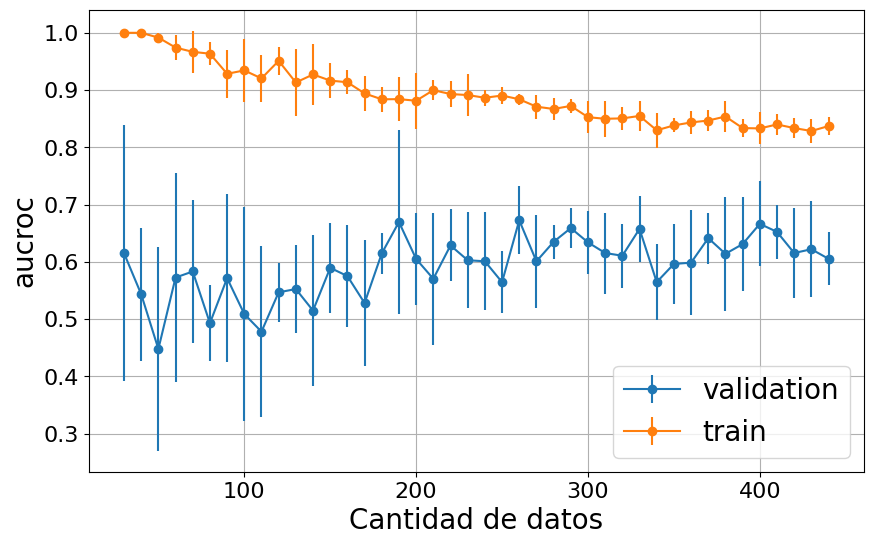
\includegraphics[width=0.75\textwidth]{/files/src/.media/decisionTreeLearning.png}
    \caption{Curvas de aprendizaje para el clasificador \textit{decision tree}, mostrando la variación del AUC ROC en datos de entrenamiento y validación a medida que se aumenta la cantidad de datos. Las lineas verticales denotan la varianza para cada tamaño de dataset.}
    \label{decisionTreeLearning}
\end{figure}


\subsection{Support vector machines}
De la Figura  que los mejores hiperparámetros para este clasificador son:

\begin{itemize}
    \item \textit{Atributos Máximos} = 135.
    \item \textit{Criterio de Corte} = Entropía.
    \item \textit{Altura Máxima} = 3
\end{itemize}

Utilizamos este último para graficar las curvas de complejidad observadas en la Figura \ref{decisionTreeComplexity}. En ellas podemos apreciar que, respaldando los resultados de este clasificador en la sección anterior, obtenemos la mejor performance utilizando \textit{altura máxima} 3 y 4. Podemos intuir que durante la búsqueda aleatoria de hiperparámentros la combinación con \textit{altura máxima} 4 no se habría probado, de otro modo hubiese aparecido como la mejor.  

\begin{figure}[!htbp]
    \centering
    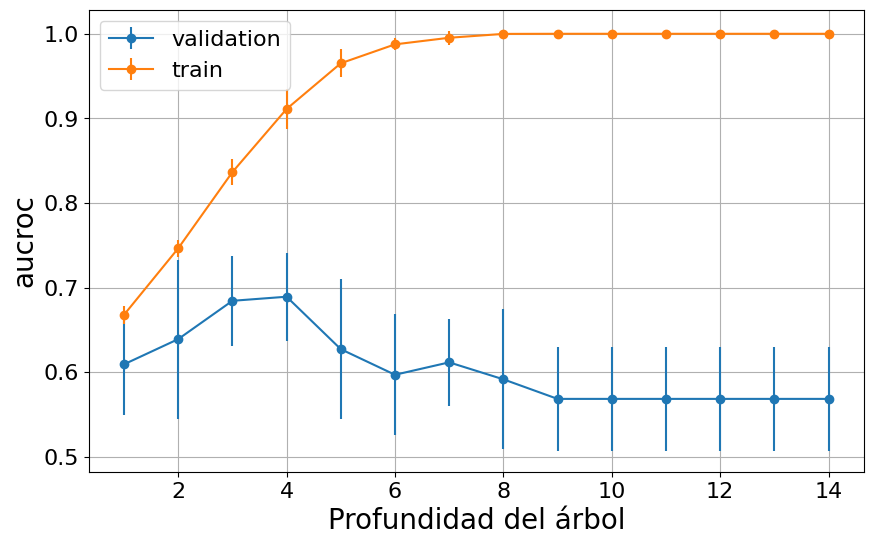
\includegraphics[width=0.75\textwidth]{/files/src/.media/decisionTreeComplexity.png}
    \caption{Curvas de complejidada para el clasificador \textit{decision tree}, mostrando la variación del AUC ROC en datos de entrenamiento y validación a medida que se aumenta su profundida máxima.}
    \label{SVMComplexity}
\end{figure}

A partir de los clasificadores de altura mayor a 7 se puede ver cómo el modelo se  acopla completamente a los datos de entrenamiento, generando un \textit{overfitting}. A su vez, sus respectivas performances en los datos de validación decrementan desde el mejor valor de \textit{altura máxima} = 4 hasta estabilizarse en las alturas mayores a 8. Esto podría indicar que el modelo ya separó todas las instancias en sus respectivas hojas, y dejó de cambiar sus reglas de corte. 

\subsection{Random forests}


\vspace{1em}
\section{Evaluación de performance}
De los resultados obtenidos a lo largo de este informe, vemos que los modelos más prometedores parecen ser aquellos basados en los algoritmos de \textit{linear discriminant analysis} y \textit{support vector machines}. En la búsqueda aleatoria ambos obtuvieron buenos puntajes. El anterior obtuvo un \textit{aucroc} promedio de $0.8649$ y el posterior de $0.8960$.

A pesar de la ventaja aparente del segundo, en el diagnóstico de sesgo y varianza continuamos por observar el comportamiento de ambos y notamos que el modelo basado en el algoritmo de \textit{support vector machines} parece tener un sesgo mayor y una tendencia a sobreajustarse a los datos, incluso al contar con una cantidad de datos grande de entrenamiento.

Luego, consideramos que el mejor modelo ---tanto en el sentido del \textit{aucroc} promedio, como en el sentido de la confianza que nuestra experimentación nos permite depositar en esta métrica--- es aquel obtenido por el algoritmo de \textit{linear discriminant analysis} con los hiperparámetros encontrados.  

Procedimos, finalmente, a entrenar un único modelo a través de este algoritmo con todos los datos de entrenamiento. Las Figuras \ref{metricas_final} y \ref{curvas_final} muestran su performance en evaluación. Estos valores conforman nuestra estimación empírica del poder de generalización del modelo.

Importa notar que hubo una pérdida de $6\%$ con repecto al mejor resultado obtenido durante validación. Sin embargo, esto es esperable, dado que la validación cruzada fue parte del proceso de entrenamiento y, por ende, da una mirada optimista de la performance real del modelo.

\vspace{0.5em}
\begin{figure}[!htbp]
    \begin{center}
        \begin{tabular}{ |c|c| } 
         \hline
        Métrica         & Valor \\
        \hline
        accuracy (test) &  0.8235 \\
        auprc (test)    &  0.7647 \\
        aucroc (test)   &  0.8321 \\
        \hline
        \end{tabular}
    \end{center}
    \caption{\textit{Accuracy}, \textit{aucroc} y \textit{auprc} obtenidos para el modelo final, evaluado sobre $D_{test}$} \label{metricas_final}
\end{figure}

\begin{figure}[!htbp]
    \centering 
    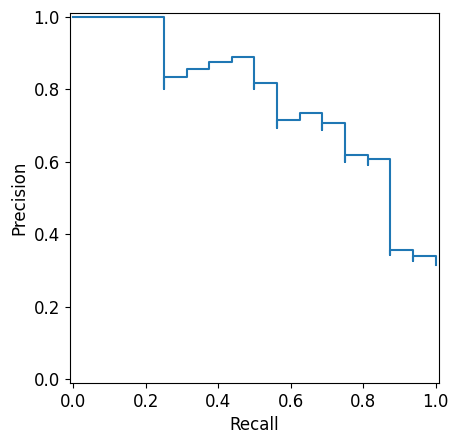
\includegraphics[width=0.45\textwidth]{/files/src/.media/finalAuprc.png}
    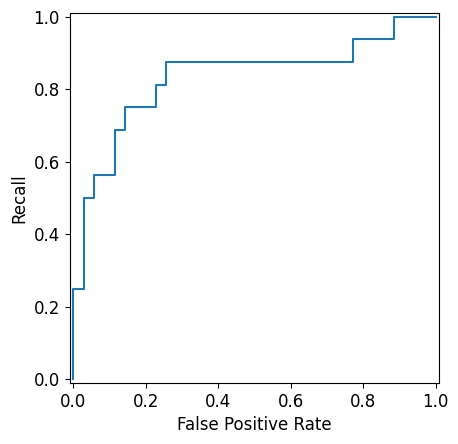
\includegraphics[width=0.45\textwidth]{/files/src/.media/finalAucroc.png}
    \caption{Curvas \textit{precision-recall}, izquierda, y \textit{receiving operator characteristic}, derecha, para el modelo final.}
    \label{curvas_final}
\end{figure}


\vspace{1em}
\section{Conclusiones}
A lo largo de este informe, experimentamos con distintos algoritmos de aprendizaje automático y evaluamos sus respectivos rendimientos. En base a los datos obtenidos, se eligió el clasificador que para nosotros mejor aproxima la solución al problema y estudiamos su performance final. 

Creemos interesante aprovechar esta sección para mencionar algunos problemas con los que nos encontramos y proponer mejoras metodológicas para futuras investigaciones.

Uno de los aspectos sobre los cuales no profundizamos fue el hecho de normalizar o no los datos. Para algunos algoritmos, tales como \textit{support vector machines} y \textit{k-nearest neighbours}, se sabe que hacerlo puede tener una implicancia importante sobre los resultados. Durante las etapas de entrenamiento y validación exploramos esta dimensión, pero optamos por no incluirla ya que no parecía mejorar los resultados. Esto podría ser un error de nuestra parte, ya que, a pesar de arrojar peores resultados, podría conducir a modelos más robustos.

A su vez, no nos enfocamos en realizar un análisis previo del dataset. Por ejemplo, investigar cómo se distribuyen los atributos. Lo único que realizamos ---de manera exploratoria--- fue un pequeño análisis basado en un resumen estadístico. En el mismo, notamos una media ---de manera general para todos los atributos--- rondando el $0$ y, a su vez, algunos indicios que reflejarían que los mismos se comportan de manera normal. Consideramos que en futuras investigaciones deberíamose realizar una exploración mayor respecto a los atributos con los que contamos, por ejemplo a través de un análisis de sus importancias.

Por otro lado, no se contempló si la métrica \textit{aucroc} promedio es la más indicada para el dominio de este problema. Por ejemplo, \cite{Saito} recomienda usar la métrica \textit{auprc} cuando la proporción de las clases es desbalanceada, como sucede en este caso. Esto está también relacionado a cuál es la clase positiva. Si bien no se investigó si convendría utilizar el \textit{mal pronóstico}, al menos sabemos que la métrica \textit{aucroc} es más imparcial respecto a cuál de las clases representa la etiqueta. Estas elecciones son muy importantes y futuras investigaciones deberían abordarlas con mayor consciencia.

Por último, vale la pena mencionar las limitaciones en la manera en que realizamos la búsqueda de los hiperparámetros. Consideramos que la cantidad de iteraciones realizada fue baja respecto a los espacios de búsqueda que decidimos explorar. A su vez, es muy posible que existan mejores métodos de sampleo que aquellos que empleamos. Otro aspecto que no fue explorado fue la posibilidad de realizar una búsqueda en cuadrícula en vez de aleatoria, sobre todo para los hiperparámetros cuyos valores son discretos. Creemos que una mejor investigación pondría mayor énfasis en los métodos a través de los cuales realizar este tipo de exploraciones.

% apendice
% \section{Apéndice}
% % TODO
% \newpage

%bibliografia - requiere que haya citas
\newpage
\bibliographystyle{plain}
\bibliography{./files/citations.bib}

\end{document}
